\documentclass[tikz,border=2pt]{standalone}
\usepackage{tikz}
\begin{document}
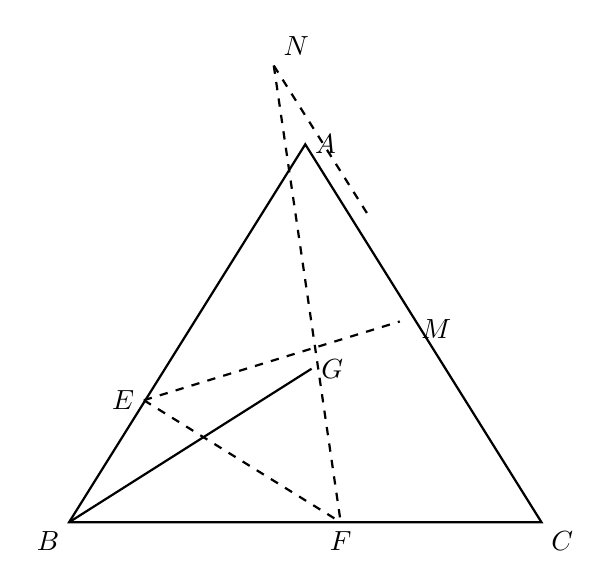
\begin{tikzpicture}[scale=1]

% Triangle
\draw[thick] (0,0) -- (3,4.8) -- (6,0) -- cycle;

% Existing dashed segments
\draw[dashed, thick] (2.6,5.8) -- (3.8,3.9);
\draw[dashed, thick] (2.6,5.8) -- (3.45,0);
\draw[dashed, thick] (0.95,1.55) -- (4.2,2.55);
\draw[dashed, thick] (0.95,1.55) -- (3.45,0);

% Added segment BG
\draw[thick] (0,0) -- (3.08,1.95);

% Labels
\node[above right] at (2.6,5.8) {$N$};
\node[right] at (3,4.8) {$A$};
\node[right] at (4.35,2.45) {$M$};
\node[left] at (0.95,1.55) {$E$};
\node[below] at (3.45,0) {$F$};
\node[below left] at (0,0) {$B$};
\node[below right] at (6,0) {$C$};
\node[right] at (3.08,1.95) {$G$};

\end{tikzpicture}
\end{document}
